% !TeX root = document.tex
% !TeX encoding = UTF-8 Unicode

\section{Introdução e Análise Exploratória}

\begin{slide}{Objetivo do Trabalho}
  \begin{itemize}
    \item Desenvolver um experimento contemplando análise e compreensão dos dados.
    \item Aplicar pré-processamento e definir uma metodologia experimental adequada.
    \item Comparar modelos de forma reprodutível e metodologicamente correta.
  \end{itemize}
\end{slide}

\begin{slide}{Contextualização do Problema}
  \begin{itemize}
    \item \textbf{Descrição:} identificação do problema associado ao conjunto de dados.
    \item \textbf{Cenário:} predição de renda anual com dados do censo de 1994.
    \item \textbf{Objetivo do modelo:} prever se a renda anual supera 50 mil dólares.
    \item \textbf{Tipo de tarefa:} classificação binária.
  \end{itemize}
\end{slide}

\begin{slide}{Caracterização Geral da Base}
  \begin{itemize}
    \item \textbf{Fonte:} UCI Machine Learning Repository.
    \item \textbf{Total de instâncias:} 32.561 registros.
    \item \textbf{Número de atributos:} 14 variáveis preditoras.
    \item \textbf{Atributos mistos:} variáveis categóricas, inteiras e reais.
  \end{itemize}

  \vspace{0.3cm}
  \scriptsize
  \begin{table}
    \centering
    \begin{tabular}{llll}
      \toprule
      age & workclass & fnlwgt & education \\
      education-num & marital-status & occupation & relationship \\
      race & sex & capital-gain & capital-loss \\
      hours-per-week & native-country &  &  \\
      \bottomrule
    \end{tabular}
    \caption{Lista de atributos da base Adult Census Income.}
  \end{table}
\end{slide}

\begin{slide}{EDA: Distribuição de Idade}
  \begin{itemize}
    \item \textbf{Método:} histogramas para visualizar concentração dos dados.
    \item \textbf{Observação:} maior parte da amostra entre 20 e 50 anos.
    \item \textbf{Importância:} compreender a demografia e reduzir vieses geracionais.
  \end{itemize}

  \begin{figure}
    \centering
    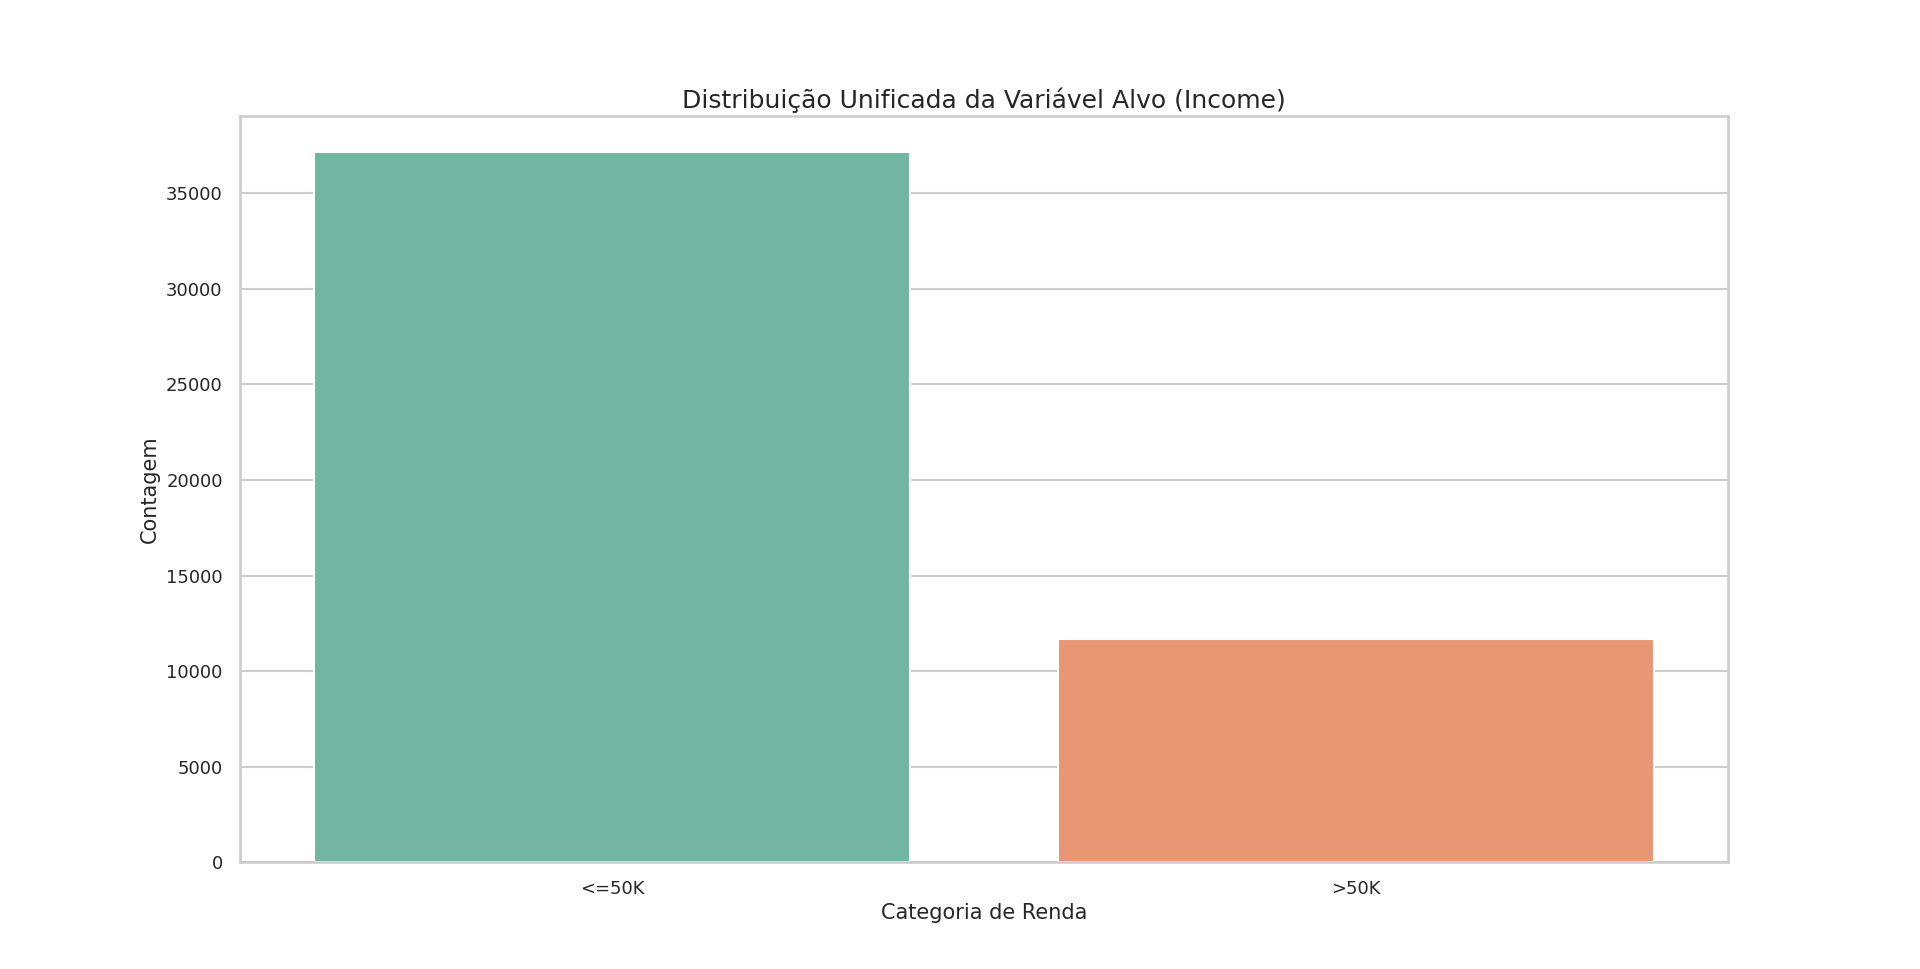
\includegraphics[width=0.72\textwidth]{../atividade_1/images/histograma.png}
    \caption{Histograma da variável idade.}
  \end{figure}
\end{slide}

\begin{slide}{EDA: Horas Trabalhadas e Renda}
  \begin{itemize}
    \item \textbf{Método:} boxplots relacionando horas semanais e classe de renda.
    \item \textbf{Outliers:} casos extremos de até 99 horas por semana.
    \item \textbf{Tendência:} renda \textgreater 50K tende a maior carga horária média.
  \end{itemize}

  \begin{figure}
    \centering
    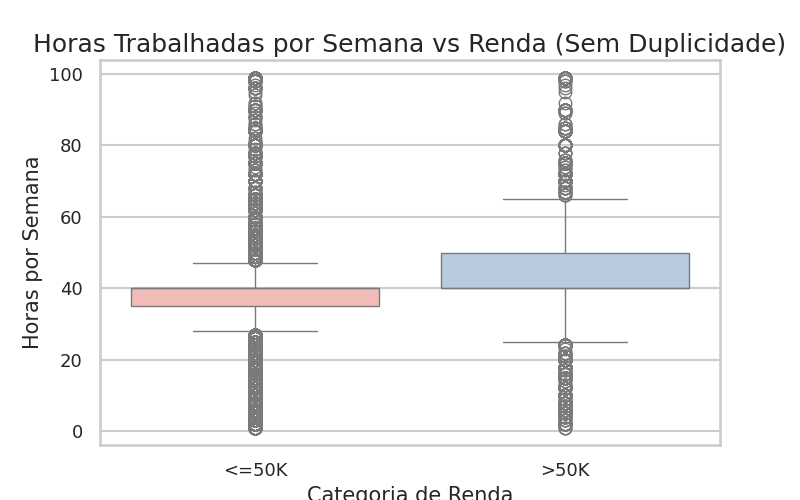
\includegraphics[width=0.72\textwidth]{../atividade_1/images/boxplot.png}
    \caption{Distribuição de horas por semana por classe de renda.}
  \end{figure}
\end{slide}

\begin{slide}{Identificação de Problemas de Qualidade}
  \begin{itemize}
    \item \textbf{Valores ausentes:} presença de ``?'' em colunas como workclass e occupation.
    \item \textbf{Ruídos de rótulo:} inconsistência entre ``\textless=50K'' e ``\textless=50K.''.
    \item \textbf{Desbalanceamento:} classe de menor renda representa aproximadamente 76\%.
    \item \textbf{Redundância:} atributo education redundante em relação ao education-num.
  \end{itemize}
\end{slide}
